\chapter{Architecture and Design}

\section*{Introduction}

This chapter will give a glimpse on the conceptual phase of our project.

\vspace{-8pt}
\enlargethispage{3cm}
\section{Dashboard}

\vspace{-5pt}
\subsection{Use Case Diagram}

\vspace{-8pt}

\begin{figure}[H]
\centering
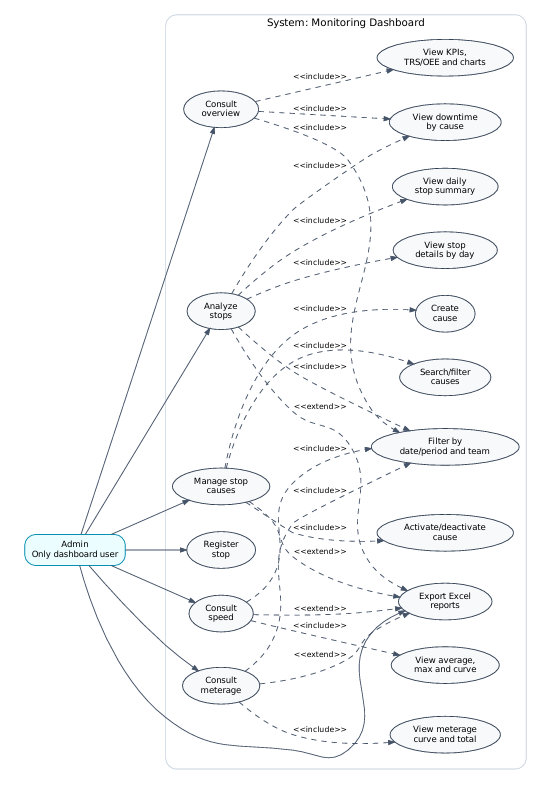
\includegraphics[width=0.6\textwidth, keepaspectratio]{images/usecase .png}
\caption{Use Case Diagram of the Dashboard}
\label{fig:chapter2-1}
\end{figure}

\subsection{Use Case Description}

\begin{table}[H]
\centering
\caption{Use Case Descriptions}
\resizebox{\textwidth}{!}{%
\begin{tabular}{|l|l|p{6cm}|}
\hline
\textbf{Use case} & \textbf{Actor} & \textbf{Description} \\
\hline
Consult overview & Admin & Select a day or period, choose a team and view global KPIs and charts. \\
\hline
Analyze stops & Admin & Consult the daily summary, select a date, view paginated stop details and analyze downtime by cause. \\
\hline
Register stop & Admin & Create a stop through the back-end with a date, start time, optional end time and optional cause. \\
\hline
Manage stop causes & Admin & Search causes, create a cause, activate or deactivate a cause and export the cause list. \\
\hline
Consult meterage & Admin & View daily meterage and period total; export the data. Creation of meterage is not modeled. \\
\hline
Consult speed & Admin & View daily average/max speed and period summary; export the data. Creation of speed is not modeled. \\
\hline
Export Excel reports & Admin & Produce Excel files for stops, causes, meterage and speed. \\
\hline
\end{tabular}%
}
\label{tab:chapter2-1}
\end{table}

\subsection{Sequence - Overview Consultation}

\begin{figure}[H]
\centering
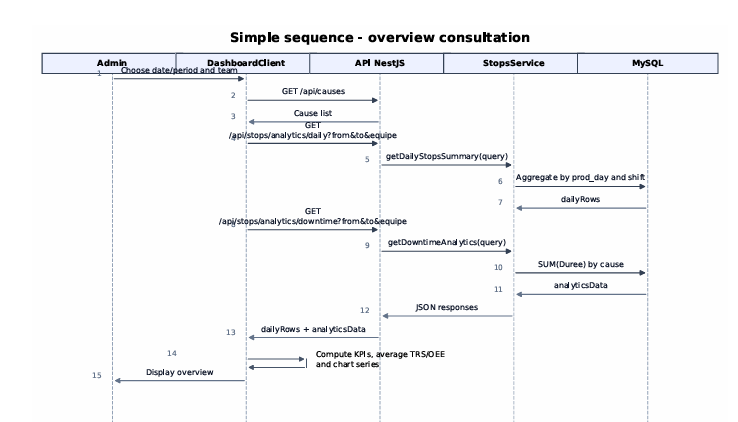
\includegraphics[width=0.85\textwidth, keepaspectratio]{images/overview consulatation.png}
\caption{Sequence Diagram: Overview Consultation}
\label{fig:chapter2-2}
\end{figure}

\subsection{Sequence - Stop Analysis and Excel Export}

\begin{figure}[H]
\centering
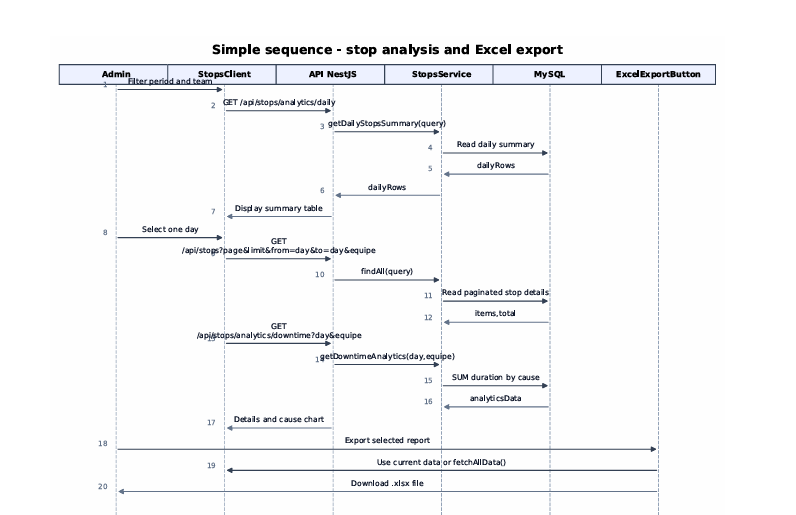
\includegraphics[width=0.85\textwidth, keepaspectratio]{images/sequance stops and export .png}
\caption{Sequence Diagram: Stop Analysis and Excel Export}
\label{fig:chapter2-3}
\end{figure}



\section{Technical Revision Context}

The machine is already installed in the workshop; therefore, the work is a CAD and documentation correction, not a new design. A mate error is treated here as a digital assembly inconsistency: failed reference, redundant constraint, over-defined relation, or wrong positioning.

The revision priorities are limited to the elements that affect technical reading, drawing extraction, and traceability. They are summarized in Table~\ref{tab:scope-revision}.

\begin{table}[H]
\centering
\small
\caption{Scope of the technical revision}
\label{tab:chapter2-2}
\resizebox{\textwidth}{!}{%
\begin{tabular}{|l|l|l|}
\hline
\textbf{Revision item} & \textbf{Technical action} & \textbf{Expected result} \\
\hline
CAD assembly mates & Correct failed, missing, redundant, or conflicting mates. & Stable rebuild with no detected mate errors. \\
\hline
Assembly organization & Keep the main machine groups in a coherent mechanical hierarchy. & Clear reading of unwinding, inspection, and rewinding functions. \\
\hline
Industrial title block & Standardize the sheet identification fields. & Traceable drawings with scale, revision, date, and validation data. \\
\hline
Technical drawing package & Prepare the useful views for the assembly, sub-assemblies, and parts. & Readable documentation for presentation, checking, and later updates. \\
\hline
\end{tabular}%
}
\end{table}

\section{Existing Machine and Functional Reference}

The CAD model must keep the same fabric path as the real machine: input roll, unwinding zone, inspection zone, rewinding zone, and output roll. This functional reference gives a clear basis for grouping parts and drawing sheets.

The three main zones are kept in the documentation because they match the real mechanical operation of the machine. This avoids mixing all components in one unclear representation.

\subsection{Complete assembly view}

The complete assembly view is used as the global CAD reference of the corrected model. It shows the complete fabric inspection machine after the mate correction, with the unwinding block, the central inspection block, and the rewinding block kept in their real functional order.

\section{CAD Assembly Correction}

\subsection{Mate review method}

The mate review targeted constraints that could affect rebuild stability or technical reading. Only mates that define the mechanical function were kept; duplicated or contradictory mates were removed.

For rotating elements, the correction focused on coherent axes. For fixed supports and frames, it focused on stable contact references and logical fixation planes.

\begin{table}[H]
\centering
\small
\caption{CAD mate correction strategy}
\label{tab:chapter2-3}
\resizebox{\textwidth}{!}{%
\begin{tabular}{|l|l|l|}
\hline
\textbf{Observed CAD condition} & \textbf{Correction approach} & \textbf{Technical purpose} \\
\hline
Failed or missing reference & Reassign the mate to a valid face, axis, plane, or reference geometry. & Restore stable positioning after rebuild. \\
\hline
Over-defined constraint & Remove duplicated or contradictory relations. & Avoid mate conflict and simplify the assembly tree. \\
\hline
Misaligned rotating element & Rebuild the concentric or coaxial relation on the correct mechanical axis. & Keep shafts, cylinders, bars, and bearings coherent. \\
\hline
Floating component & Add only the minimum functional constraints. & Prevent unintended movement without over-constraining the model. \\
\hline
Incorrect sub-assembly position & Reposition the group using stable references from the main structure. & Preserve the real machine architecture. \\
\hline
\end{tabular}%
}
\end{table}

\subsection{Final assembly validation}

After correction, the assembly was rebuilt and checked. The validation was not limited to visual appearance; it also required a clean mate status, coherent axes, correct sub-assembly positions, and readiness for drawing extraction.

\begin{table}[H]
\centering
\small
\caption{Final CAD assembly validation criteria}
\label{tab:chapter2-4}
\resizebox{\textwidth}{!}{%
\begin{tabular}{|l|l|l|}
\hline
\textbf{Validation criterion} & \textbf{Requirement} & \textbf{Expected result} \\
\hline
Mate status & No detected failed, dangling, or conflicting mates. & Clean assembly tree and reliable rebuild. \\
\hline
Component positioning & Main parts placed according to the real machine structure. & Correct visual interpretation of the layout. \\
\hline
Rotating axes & Cylinders, shafts, bearings, and bars aligned with coherent axes. & Consistent representation of rotating elements. \\
\hline
Sub-assembly hierarchy & Functional groups remain identifiable. & Clear reading of unwinding, inspection, and rewinding zones. \\
\hline
Drawing extraction readiness & Views generated from stable references. & Reliable basis for the technical drawing package. \\
\hline
\end{tabular}%
}
\end{table}

\section{Industrial Title Block Standardization}

The title block was standardized so that each sheet can be identified without returning to the complete report. It gives the drawing its basic traceability: project, part or assembly name, drawing number, scale, revision, date, drafter, checker, and sheet number.

\begin{table}[H]
\centering
\small
\caption{Main fields of the revised industrial title block}
\label{tab:chapter2-5}
\resizebox{\textwidth}{!}{%
\begin{tabular}{|l|l|l|}
\hline
\textbf{Title-block field} & \textbf{Role} & \textbf{Reason for inclusion} \\
\hline
Project or machine name & Identifies the global system. & Links the sheet to the fabric inspection machine. \\
\hline
Part or assembly name & Identifies the represented element. & Avoids confusion between similar components. \\
\hline
Drawing number & Gives a unique sheet reference. & Supports classification and retrieval. \\
\hline
Scale and sheet format & Defines representation conditions. & Makes the sheet easier to read and check. \\
\hline
Revision, date, drafter, checker & Records the current version and validation status. & Improves traceability and responsibility tracking. \\
\hline
\end{tabular}%
}
\end{table}

\section{Technical Drawing Package}

\subsection{Drawing package organization}

The drawing package is organized by level: complete assembly, functional sub-assemblies, and individual parts. This avoids overloaded sheets and gives each drawing a precise technical purpose.

\begin{table}[H]
\centering
\small
\caption{Organization of the technical drawing package}
\label{tab:chapter2-6}
\resizebox{\textwidth}{!}{%
\begin{tabular}{|l|l|l|}
\hline
\textbf{Drawing level} & \textbf{Main content} & \textbf{Technical objective} \\
\hline
Complete assembly drawing & Overall machine view, main zones, and principal components. & Present the corrected machine as a complete system. \\
\hline
Sub-assembly drawings & Separate views for unwinding, inspection, and rewinding groups. & Clarify the role and location of each functional zone. \\
\hline
Individual part drawings & Orthographic, section, detail, or isometric views as needed. & Identify each part and its useful geometry. \\
\hline
Title-block information & Drawing number, name, scale, revision, date, and validation fields. & Ensure traceability and professional presentation. \\
\hline
\end{tabular}%
}
\end{table}

The CAD views for the chapter are named according to their mechanical function: complete assembly, unwinding unit, inspection unit, and rewinding unit. This naming keeps the drawing package readable because each view is linked to one clear documentation level instead of being treated as an isolated render.

\subsection{Required views for the parts}

The selected views must explain the geometry without unnecessary visual overload. Simple parts can be described with orthographic and isometric views; complex parts need sections or details when hidden geometry and interfaces are not clear.

\begin{table}[H]
\centering
\small
\caption{Recommended view selection for the drawing sheets}
\label{tab:chapter2-7}
\resizebox{\textwidth}{!}{%
\begin{tabular}{|l|l|l|}
\hline
\textbf{Component type} & \textbf{Recommended views} & \textbf{Purpose of the views} \\
\hline
Complete assembly & General 3D view, front view, side view, and overall layout. & Show the complete machine and the main zones. \\
\hline
Functional sub-assembly & Isometric view, principal orthographic views, and local details if required. & Clarify composition and mechanical role. \\
\hline
Shafts, cylinders, and bars & Longitudinal view, end view, and interface detail if needed. & Show axes, diameters, ends, and mounting interfaces. \\
\hline
Supports, brackets, and plates & Front, top, side, and section views where necessary. & Make holes, thicknesses, fixing areas, and contact faces readable. \\
\hline
Moving or adjustable elements & Main view, position reference view, and connection detail. & Show mounting logic and adjustment interface. \\
\hline
\end{tabular}%
}
\end{table}

\section{Mechanical Reading After Correction}

The corrected documentation should allow the reader to follow the fabric path and locate the main mechanical groups quickly. Each zone must therefore show only the elements needed to understand its function.

\begin{table}[H]
\centering
\small
\caption{Mechanical reading after CAD correction}
\label{tab:chapter2-8}
\resizebox{\textwidth}{!}{%
\begin{tabular}{|l|l|l|}
\hline
\textbf{Machine zone} & \textbf{Elements to represent clearly} & \textbf{Documentation objective} \\
\hline
Unwinding zone & Input roll, expandable bar, bearings, drive elements, supports, and first guides. & Explain how the fabric is released and introduced into the machine. \\
\hline
Inspection zone & Guide cylinders, de-wrinkling device, inspection table, lighting support, and controls. & Show how the fabric is presented for visual inspection. \\
\hline
Rewinding zone & Output roll, expandable bar, drive elements, guide cylinders, actuators, and adjustment elements. & Explain how the inspected fabric is recovered into the final roll. \\
\hline
\end{tabular}%
}
\end{table}

\subsection{CAD views of the functional blocks}

The following CAD views serve as sub-assembly references for understanding the functional blocks.

\subsubsection{Unwinding Unit -- Input Roll and Drive Support}

The unwinding unit represents the inlet side of the machine. It supports the fabric roll, keeps the roll axis aligned, and links the roll to the drive and bearing supports. The isolated view makes the input roll, support frame, coupling area, and first guiding direction easier to identify.

\begin{figure}[H]
\centering
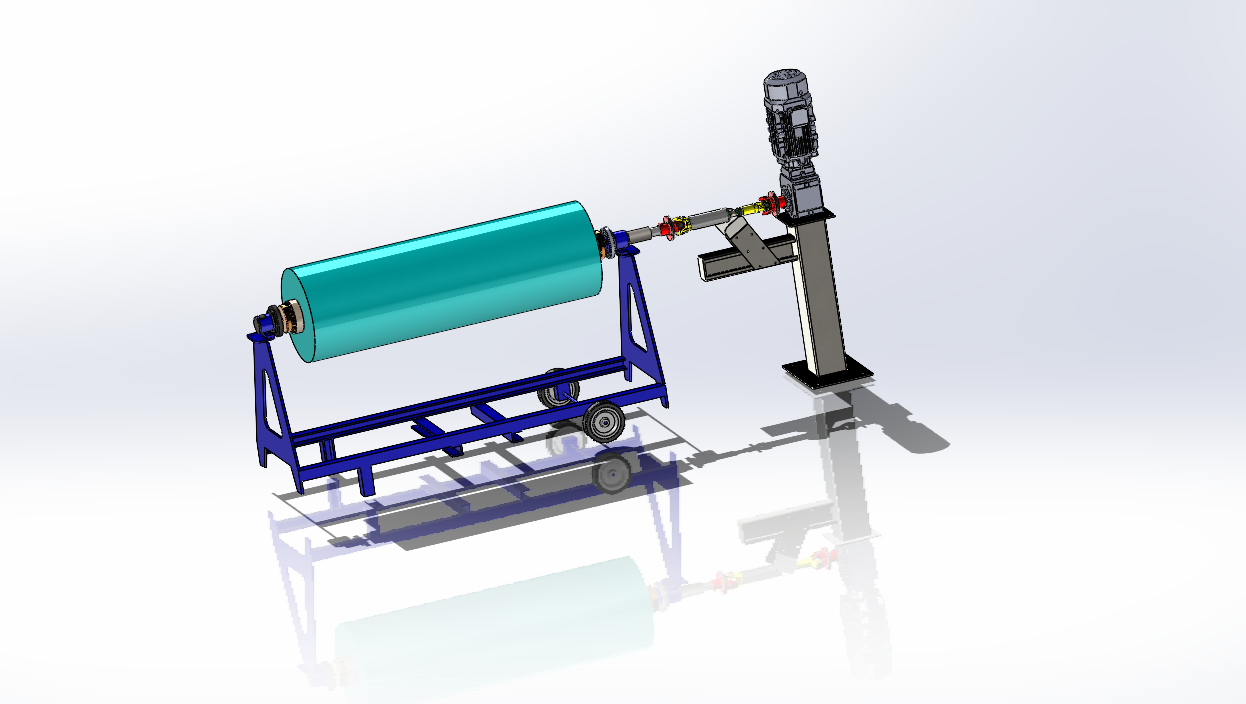
\includegraphics[width=0.8\textwidth, keepaspectratio]{images/unwinding_unit_input_roll_drive_support.png}
\caption{Unwinding Unit -- Input Roll and Drive Support}
\label{fig:chapter2-4}
\end{figure}

\subsubsection{Inspection Unit -- Central Viewing and Guiding Section}

The inspection unit is the central working area of the machine. It contains the main guiding rollers, the inspection opening, the support structure, and the elements that keep the fabric visible and correctly guided during checking.

\begin{figure}[H]
\centering
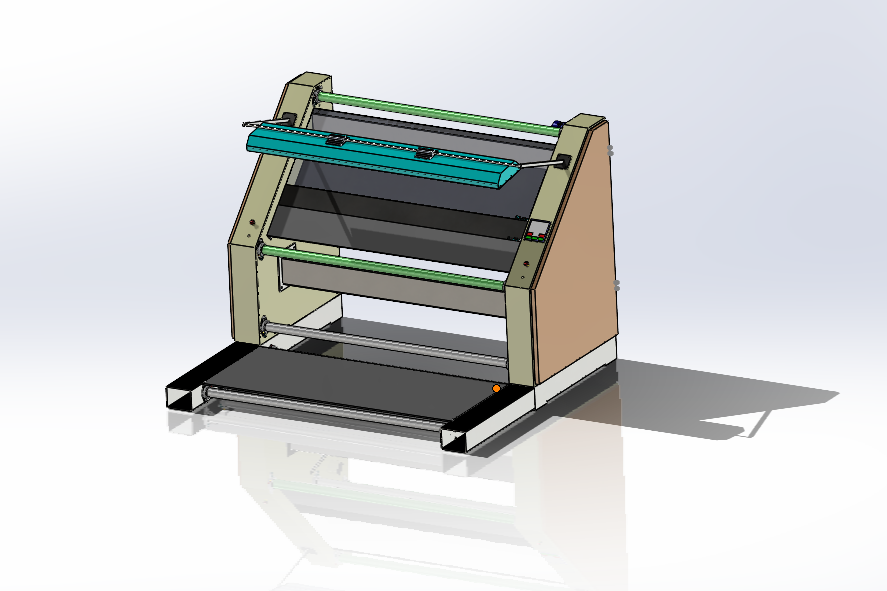
\includegraphics[width=0.8\textwidth, keepaspectratio]{images/inspection_unit_central_viewing_guiding_section.png}
\caption{Inspection Unit -- Central Viewing and Guiding Section}
\label{fig:chapter2-5}
\end{figure}

\subsubsection{Rewinding Unit -- Output Roll and Take-up Drive}

The rewinding unit represents the output side of the machine. It receives the inspected fabric and winds it onto the final roll. The view highlights the take-up roll, drive support, bearing area, and connection with the previous guiding path.

\begin{figure}[H]
\centering
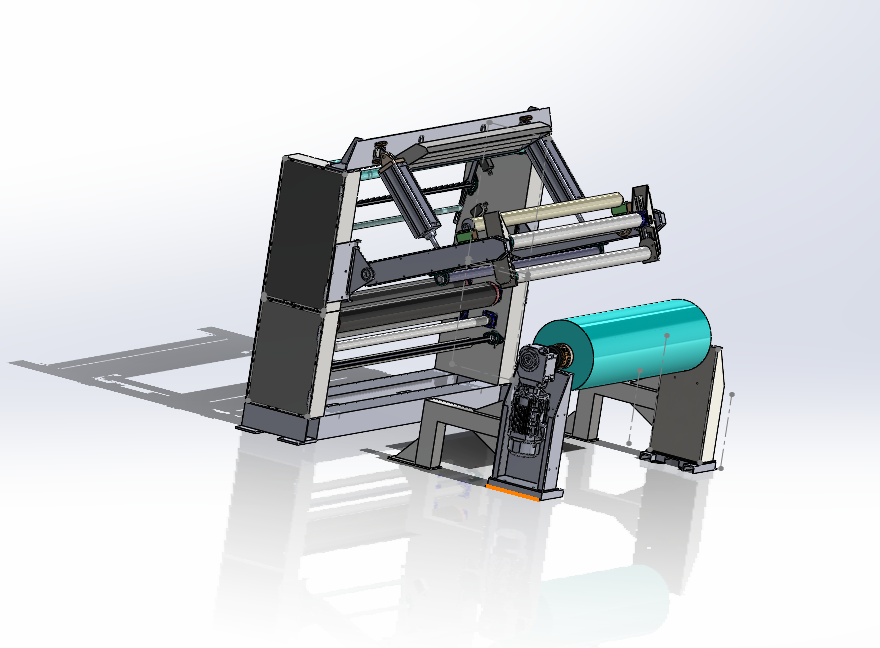
\includegraphics[width=0.8\textwidth, keepaspectratio]{images/rewinding_unit_output_roll_take_up_drive.png}
\caption{Rewinding Unit -- Output Roll and Take-up Drive}
\label{fig:chapter2-6}
\end{figure}

\section{Conclusion}

The revision produced a cleaner CAD assembly, a coherent functional organization, and a standardized drawing package. The mate structure was checked for reliable rebuild and drawing extraction. The documentation improvements ensure traceability and readability.